% !TeX spellcheck = en_US
\chapter{Actor-Critic}
Actor-Critic is kind of hybrid between policy gradient and value function based approach. Compared to deep Policy gradient, deep Actor-Critic has an extra network to learn the value function (the green box in \figref{fig:RL-structure}).
\begin{itemize}
	\item \hlr{the Actor is the policy}
	\item \hlr{the Critic is the value function (\ac{aka} policy evaluation)}
\end{itemize}

\section{Approach}
We continue with the \eqref{eq:Q-value}, where we multiply with the estimate of the expected reward $\widehat{Q}_{i,t}$. The estimate $\widehat{Q}_{i,t}$ is currently calculated as the sum of the reward afterward, in a single run. There are different ways we could go better than that single-sample estimate.

\begin{itemize}
	\item $Q^\pi(\textbf{s}_t, \textbf{a}_t)$: the Q-function, \ac{aka}, the state-action value function, represents the total reward from taking $\textbf{a}_t$ at state $\textbf{s}_t$, the \textit{true expected} reward-to-go.
	\begin{equation}
		Q^\pi(\textbf{s}_t, \textbf{a}_t) = \sum_{t'=t}^T \mathbb{E}_{\pi_{\theta}}[r(\textbf{s}_{t'}, a_{t'})|\textbf{s}_t, \textbf{a}_t]
		\label{eq:q-function}
	\end{equation}
	\item $V^\pi(\textbf{s}_t)$: the state value function represents the total reward from state $\textbf{s}_t$.
	\begin{equation}
		V^\pi(\textbf{s}_t) = \mathbb{E}_{\textbf{a}_t \sim \pi_{\theta}(\textbf{a}_t, \textbf{s}_t)} [Q^\pi(\textbf{s}_t, \textbf{a}_t)]
	\end{equation}
	\item $A^\pi(\textbf{s}_t, \textbf{a}_t)$: the advantage function: represents how much action $\textbf{a}_t$ is better than average
	\begin{equation}
		A^\pi(\textbf{s}_t, \textbf{a}_t) = Q^\pi(\textbf{s}_t, \textbf{a}_t) - V^\pi(\textbf{s}_t)
		\label{eq:a-function}
	\end{equation}
\end{itemize}

Using these value functions, we would have a better estimate for the policy gradients. Thus, we can rewrite the gradient as:
\begin{align}
	\nabla_\theta J(\theta) &= \frac{1}{N} \sum_{i=1}^N\sum_{t=1}^T \nabla_\theta\log\pi_{\theta}( \textbf{a}_{i,t}|\textbf{s}_{i,t} ) A^\pi(\textbf{s}_{i,t}, \textbf{a}_{i,t} )\\
	Q^\pi(\textbf{s}_t, \textbf{a}_t) &= r(\textbf{s}_t, \textbf{a}_t) + \mathbb{E}_{\textbf{s}_{t+1}\sim p(\textbf{s}_{t+1} | \textbf{s}_t, \textbf{a}_t)} V^\pi(\textbf{s}_{t+1}) && \text{(\eqref{eq:q-function})}\\
	&\approx r(\textbf{s}_t, \textbf{a}_t) + V^\pi(\textbf{s}_{t+1}) &&\text{(with 1 sample)}\\
	\Rightarrow \quad A^\pi(\textbf{s}_t, \textbf{a}_t) &\approx r(\textbf{s}_t, \textbf{a}_t) + V^\pi(\textbf{s}_{t+1}) - V^\pi(\textbf{s}_t) && \text{(\eqref{eq:a-function})}	
\end{align}

\begin{figure}[hbt!]
	\centering
	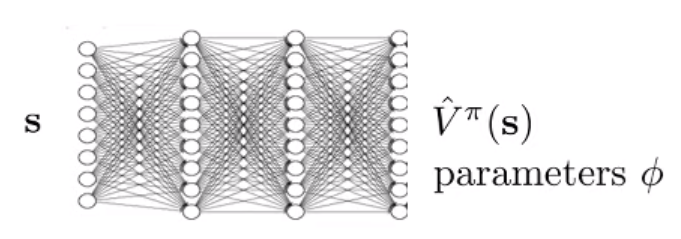
\includegraphics[width=.7\textwidth]{actor-critic.png}
	\caption{The network for value function $V_{\phi}^\pi(s)$ with \ac{param} $\phi$.}
	\label{fig:actor-critic}
\end{figure}

From the above derivation, let just fit the value function $V^\pi(\textbf{s})$ with a neural network. There are two possible approaches:
\begin{itemize}
	\item \hlr{Monte-Carlo:} just as with policy gradient, we approximate by the result from a single sample roll-out.
	\begin{equation}
		V^\pi(\textbf{s}_t) \approx \sum_{t'=t}^T r(\textbf{s}_{t'}, \textbf{a}_{t'})
	\end{equation}
	The average of multiple samples would be a better approximation for the true expectation. However, we could not simply stop at one state within the trajectories and try out different actions. Single sample estimation is still pretty good!
	\begin{align}
		&\text{Better (but not possible)} && V^\pi(\textbf{s}_t) \approx \frac{1}{N} \sum_{i=1}^N \sum_{t'=t}^T r(\textbf{s}_{t'}, \textbf{a}_{t'})\\
		&\text{Training data:} && \{(\textbf{s}_{i,t}, y_{i,t}) \} = \left\{\left(\textbf{s}_{i,t}, \sum_{t'=t}^T r(\textbf{s}_{i,t'}, \textbf{a}_{i,t'})\right)\right\}\\
		&\text{Supervised regression:} && \mathcal{L}(\phi) = \frac{1}{2} \sum_{i} \left|\left| \widehat{V}_{\phi}^{\pi}(\textbf{s}_i) - y_i\right|\right| ^2
	\end{align}
	\item \hlr{Bootstrapped estimate:} use the previous fitted value function
	\begin{align}
		y_{i,t} &= \sum_{t'=t}^{T} \mathbb{E}_{\pi_{\theta}} [r(\textbf{s}_{t'}, a_{t'} | \textbf{s}_{i,t})] &&\text{ideal target}\\
		&\approx r(\textbf{s}_{i,t}, a_{i, t}) + V^{\pi}(\textbf{s}_{i,t+1})\\
		&\approx r(\textbf{s}_{i,t}, a_{i, t}) + \widehat{V}_{\phi}^{\pi}(\textbf{s}_{i,t+1})
	\end{align}
	\begin{align}
		&\text{Training data:} && \{(\textbf{s}_{i,t}, y_{i,t}) \} = \left\{\left(\textbf{s}_{i,t}, r(\textbf{s}_{i,t}, \textbf{a}_{i,t}) + \widehat{V}^\pi_\phi(\textbf{s}_{i,t+1}) \right)\right\}\\
		&\text{Supervised regression:} && \mathcal{L}(\phi) = \frac{1}{2} \sum_{i} \left|\left| \widehat{V}_{\phi}^{\pi}(\textbf{s}_i) - y_i\right|\right| ^2
	\end{align}	
\end{itemize}

\section{Batch Actor-Critic}
\begin{enumerate}
	\item \tikzmark{bac1}Sample $\{\textbf{s}_i, \textbf{a}_i\}$ from $\pi_{\theta}(\textbf{a|s})$
	\item Fit $V_{\phi}^\pi(\textbf{s})$ to sampled reward sums (either Monte-Carlo or bootstrapped estimate)
	\item Evaluate $\widehat{A}^\pi(\textbf{s}_i, \textbf{a}_i) = r(\textbf{s}_i, \textbf{a}_i) + \widehat{V}_\phi^\pi(\textbf{s}_{i'}) - \widehat{V}_\phi^\pi(\textbf{s}_{i})$
	\item $\nabla_\theta J(\theta) \approx \sum \nabla_\theta\log\pi_{\theta}( \textbf{a}_{i}|\textbf{s}_{i} ) \widehat{A}^\pi(\textbf{a}_i, \textbf{s}_i)$
	\item \tikzmark{bac5}$\theta \leftarrow \theta + \alpha \nabla_\theta J(\theta)$
	\begin{tikzpicture}[overlay,remember picture]
		\draw[very thick, -latex] ([xshift=-7mm,yshift=1mm]pic cs:bac5) --++ (-.5,0) |- ([xshift=-7mm,yshift=1mm]pic cs:bac1);
	\end{tikzpicture}
\end{enumerate}
With \hlr{discount factor $\gamma$} $\in [0,1]$ (0.99 works well)\\
3. Evaluate $\widehat{A}^\pi(\textbf{s}_i, \textbf{a}_i) = r(\textbf{s}_i, \textbf{a}_i) + \gamma\widehat{V}_\phi^\pi(\textbf{s}_{i'}) - \widehat{V}_\phi^\pi(\textbf{s}_{i})$ \cite{thomas2014icml}

\section{Online Actor-Critic}
\begin{enumerate}
	\item \tikzmark{oac1}Take action $\textbf{a} \sim \pi_{\theta}(\textbf{a|s})$, get sample $(\textbf{s, a, s'}, r)$
	\item Update $\widehat{V}_\phi^\pi$ using target value $r + \gamma \widehat{V}_\phi^\pi(\textbf{s}')$
	\item Evaluate $\widehat{A}^\pi(\textbf{s, a}) = r(\textbf{s, a}) + \widehat{V}_\phi^\pi(\textbf{s}') - \widehat{V}_\phi^\pi(\textbf{s})$
	\item $\nabla_\theta J(\theta) \approx \nabla_\theta\log\pi_{\theta}(\textbf{a|s}) \widehat{A}^\pi(\textbf{s, a})$
	\item \tikzmark{oac5}$\theta \leftarrow \theta + \alpha \nabla_\theta J(\theta)$
	\begin{tikzpicture}[overlay,remember picture]
		\draw[very thick, -latex] ([xshift=-7mm,yshift=1mm]pic cs:oac5) --++ (-.5,0) |- ([xshift=-7mm,yshift=1mm]pic cs:oac1);
	\end{tikzpicture}
\end{enumerate}
\hlr{Problem:} single batch $\Rightarrow$ need parallel actor-critic (synchronous / asynchronous)

\section{Design Decisions}
\begin{itemize}
	\item Architecture design:
	\begin{table}[hbt!]
		\centering
		\begin{tabular}{c|c}
			Two separate networks & Shared network design\\
			\hline\hline
			$\begin{matrix*}[l]
				\color{Green} + \text{simple and stable}\\
				\color{red} - \text{no shared features between actor \& critic}
			\end{matrix*}$ & $\begin{matrix*}[l]
				\color{Green} + \text{could be more efficient in practice}\\
				\color{red} - \text{two different gradients which need to tuned}
			\end{matrix*}$ \\ 
			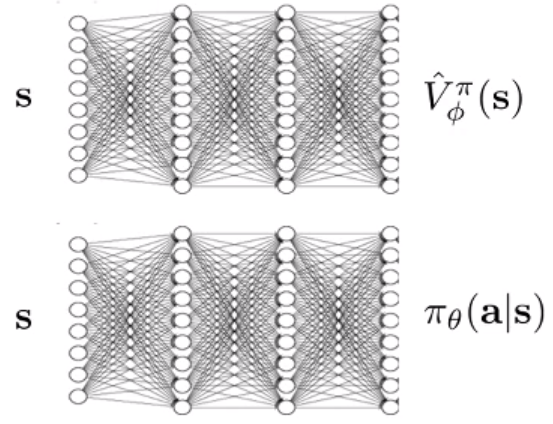
\includegraphics[width=0.3\textwidth]{ac-networks-1.png} &
			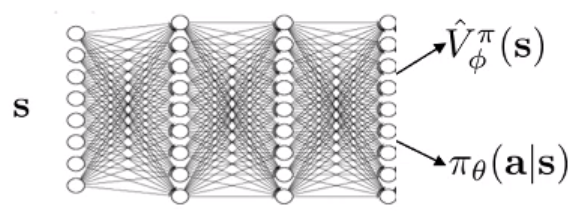
\includegraphics[width=0.5\textwidth]{ac-networks-2.png}
		\end{tabular}
	\end{table}	
	
	\item Critic as state-dependent baselines\\
	Actor-critic: $\begin{matrix*}[l]
		\color{Green}+\text{lower variance (due to critic)}\\
		\color{red}-\text{not unbiased (if the critic is not perfect)}
	\end{matrix*}$
	\[\nabla_\theta J(\theta) \approx \frac{1}{N} \sum_{i=1}^N \sum_{t=1}^T \nabla_\theta\log\pi_{\theta}(\textbf{a}_{i,t}|\textbf{s}_{i,t}) \left( r(\textbf{s}_{i,t}, \textbf{a}_{i,t}) + {\color{red}\gamma\widehat{V}_\phi^\pi(\textbf{s}_{i,t+1}) - \widehat{V}_\phi^\pi(\textbf{s}_{i,t})} \right)\]
	Policy gradient: $\begin{matrix*}[l]
		\color{Green}+ \text{no bias}\\
		\color{red}- \text{higher variance (because of single-sample estimate)}
	\end{matrix*}$
	\[\nabla_\theta J(\theta) \approx \frac{1}{N} \sum_{i=1}^N \sum_{t=1}^T \nabla_\theta\log\pi_{\theta}(\textbf{a}_{i,t}|\textbf{s}_{i,t}) \left( \left( \sum_{t' = t}^T \gamma^{t'-t} r(\textbf{s}_{i,t'}, \textbf{a}_{i,t'}) \right) -b \right)\]
	$\Rightarrow$ Critic as baseline: $\color{Green}\begin{matrix*}[l]
		+ \text{no bias}\\
		+ \text{lower variance (baseline is closer to rewards)}
	\end{matrix*}$
	\[\nabla_\theta J(\theta) \approx \frac{1}{N} \sum_{i=1}^N \sum_{t=1}^T \nabla_\theta\log\pi_{\theta}(\textbf{a}_{i,t}|\textbf{s}_{i,t}) \left( \left( \sum_{t' = t}^T \gamma^{t'-t} r(\textbf{s}_{i,t'}, \textbf{a}_{i,t'}) \right) - {\color{red}\widehat{V}_\phi^\pi(\textbf{s}_{i,t})} \right)\]
	This doesn't lower the variance as much as in the actor-critic algorithm. But it is much lower than using a constant baseline, and it's still unbiased.
	
	\item Control variates: action-dependent baselines \cite{gu2016q}\\
	We could go further with a state dependent baseline, and have a action-and-state-dependent baselines. The variance is now even lower, but it's getting much more complicated.
	\begin{align*}
		&\widehat{A}^\pi(\textbf{s}_t, \textbf{a}_t) = \sum_{t' = t}^\infty \gamma^{t'-t} r(\textbf{s}_{t'}, \textbf{a}_{t'}) - {\color{red} V_\phi^\pi(\textbf{s}_{t})} && \begin{matrix*}[l]
			\color{Green} + \text{no bias (state dependent baseline)}\\
			\color{red} - \text{still high variance (compared to actor-critic)}
		\end{matrix*}\\
		&\widehat{A}^\pi(\textbf{s}_t, \textbf{a}_t) = \sum_{t' = t}^\infty \gamma^{t'-t} r(\textbf{s}_{t'}, \textbf{a}_{t'}) - {\color{red} Q_\phi^\pi(\textbf{s}_{t}, \textbf{a}_{t})} && \begin{matrix*}[l]
			\color{Green} + \text{goes to 0 in expectation if critic is correct}\\
			\color{red} - \text{not correct}
		\end{matrix*}
	\end{align*}
	The second one lead to wrong policy gradient, thus must be corrected with an error term:
	\begin{equation}
		\nabla_\theta J(\theta) \approx \frac{1}{N} \sum_{i=1}^N \sum_{t=1}^T \nabla_\theta\log\pi_{\theta}(\textbf{a}_{i,t}|\textbf{s}_{i,t}) \left( \widehat{Q}_{i,t} - Q^\pi_\phi(\textbf{s}_{i,t}, \textbf{a}_{i,t}) \right) + \frac{1}{N} \sum_{i=1}^N \sum_{t=1}^T \nabla_\theta\mathbb{E}_{\textbf{a}\sim\pi_\theta(\textbf{a}_t | \textbf{s}_{i,t})}[Q^\pi_\phi(\textbf{s}_{i,t}, \textbf{a}_{i,t})]
	\end{equation}
	
	\item Eligibility traces \& $n$-step returns: reduces the bias
	\begin{align}
		&\text{Actor-critic:} &&\widehat{A}_C^\pi(\textbf{s}_t, \textbf{a}_t) = r(\textbf{s}_t, \textbf{a}_t) + \gamma \widehat{V}_\phi^\pi(\textbf{s}_{t+1}) - \widehat{V}_\phi^\pi(\textbf{s}_t) \quad \begin{matrix*}[l]
			{\color{Green} + \text{low variance}}\\
			{\color{red} - \text{but biased}}
		\end{matrix*}\\
		&\text{Monte-Carlo:} &&\widehat{A}_{MC}^\pi(\textbf{s}_t, \textbf{a}_t) = \sum_{t' = t}^\infty \gamma^{t'-t} r(\textbf{s}_{t'}, a_{t'}) - \widehat{V}_\phi^\pi(\textbf{s}_t) \quad\begin{matrix*}[l]
			{\color{Green} + \text{no bias}}\\
			{\color{red} - \text{higher variance}}				
		\end{matrix*}\\
		&\qquad\Rightarrow &&\widehat{A}_n^\pi (\textbf{s}_t, \textbf{a}_t) = \sum_{t'=t}^{\color{red} t+n} \gamma^{t'-t} r(\textbf{s}_{t'}, a_{t'}) - \widehat{V}_\phi^\pi(\textbf{s}_t) + \gamma^n \widehat{V}_\phi^\pi(\textbf{s}_{t+n})
	\end{align}
	Simply put, the further the states are in the future, the higher the variance of those states. \Eg, where would you/the robot be in 5 minutes versus where would you/the robot be in 20 years? The larger $n$ is, the lower the bias, the higher the variance.
	\item Generalized advantage estimation: extension of $n$-step returns\\
	To have many $n$-step returns, then take weighted average of them.	
	\begin{align}
		&\widehat{A}_{GAE}^\pi(\textbf{s}_t, \textbf{a}_t) = \sum_{n=1}^\infty \omega_n \widehat{A}_n^\pi(\textbf{s}_t, \textbf{a}_t), && \omega_n \propto \lambda^{n-1}\\
		\Rightarrow\;&\widehat{A}_{GAE}^\pi(\textbf{s}_t, \textbf{a}_t) = \sum_{t'=t}^\infty (\gamma\lambda)^{t'-t} \delta_{t'}, && \delta_{t'} = r(\textbf{s}_{t'}, \textbf{a}_{t'}) + \gamma \widehat{V}^\pi_\phi(\textbf{s}_{t'+1}) - \widehat{V}_\phi^\pi(\textbf{s}_{t'})
	\end{align}
\end{itemize}

\section{References}
\begin{itemize}
	\item \citeaus{sutton1999policy}. Policy gradient methods for reinforcement learning with function approximation.
	\item \citeausm{mnih2016icml}. Asynchronous methods for deep reinforcement learning.
	\item \citeausm{schulman2015high}. High-dimensional continuous control using generalized advantage estimation.
	\item \citeausm{gu2016q}. Q-prop: Sample-efficient policy gradient with an off-policy critic.
\end{itemize}